\pagestyle{fancy}
\fancyhf{}
\fancyfoot[L]{\textbf{ECEN 4638--T.D. Murphey}}
\fancyfoot[R]{\textbf{Lab \#3}}
\fancyfoot[C]{\vspace{.2in}\thepage}

\chapter{Lab \#3:  System Identification of the Torsional Disk System}

\begin{center}  \textbf{Objective}
\end{center}

The purpose of this lab is to familiarize you with the functioning of the EPS
Torsional Disk System (TDS) and learn how to perform a system identification on
it.  You have already done a somewhat heuristic version of this in the previous
lab--this time you will systematically identify the parameters--in particular
the parameters you cannot compute beforehand based on physical principles (e.g.,
the torsional spring constants, the inertia of the disk, and the dissipation
constants).  You will also need to establish the hardware gain for the system.
Note that it will serve you well to be familiar with this process--the four ECP
units are somewhat different from each other and will typically change their
parametric values over time, so you may find that you need to re-identify these
systems as the lab progresses.  (Hopefully you will not need to, however.)


%\vspace{.2in}

\begin{center} \textsc{Note that this lab will be a two-week lab.}
\end{center}

%\begin{center} \textsc{Also note that this lab may be updated, so please look at
%    the most recent copy before starting the lab.}
%\end{center}

\Large
\begin{center} \textsc{Warning:} 
\end{center}
\normalsize

Please do not break the TDS systems.  If you have questions, or are unsure of a
next step, please let us know.  However, the most important things are:
\begin{enumerate}
\item \emph{never run the system while it is clamped down}!  If you follow this one
rule, it is extremely unlikely (though sadly not impossible) that you will break
the system;  
\item do not twist the disks more than 30 degrees relative to each other as you
  can damage the torsional rod this way as well.
\end{enumerate}



\newpage
\section{Pre-Lab Tasks}

These tasks must be completed and (the concrete portions) shown to either the TA
or the instructor before you may use the hardware.

\noindent \textbf{Task:}  Read this entire document.

\noindent \textbf{Task:}  Create a VI that allows you to write data to a file.
Create another one that allows you to read the data and plot it.  Refer to
Section~\ref{sec-saveread} for details on how to do this.

\noindent \textbf{Task:}  We will provide you with the VI infrastructure for talking
to the hardware.  Create a single pulse using signal generation tools from the
simulation module.

\noindent \textbf{Task:}  Model the bottom and top disk as  second order systems
assuming that the middle disk is clamped down.  (You will clamp the middle disk
while doing the system identification, so you will need this model.)

\noindent \textbf{Task:}  Write down the impulse response of the bottom disk and
the top disk.  What does this correspond to physically?  Can you simulate it?
Can you experimentally produce the impulse response?

\section{Tasks}





\subsection{Task \#1--Using the Hardware}

There are a number of tasks here that have to be done during the system
identification process.  The basic idea is that you will clamp the middle disk
in order to separate the dynamics of the top disk from the bottom disk.  You
will then estimate the spring constants $k_1$ and $k_2$ by looking at the period
of oscillation and you will estimate the dissipation constants by looking at the
decay envelope of the system as oscillations die out.  First, however, you need
to be sure you can get data for the system.

\begin{enumerate}
\item Clamp the center disk and keep the hardware controller \emph{turned off}.
\item Put four masses on both the top and bottom disks 9.0 cm away from the center of
  the disk.  (The rings in the disk are 1.0 cm apart.)
\item Test that you can read all three encoder values for a 10 second time
  period.  
\item When you start the experiment in LabVIEW, the encoder should automatically
  zero so that all the encoders are at zero.  Let us know if they don't.  
\item Plot the output of one of the encoders.  Keep in mind that the encoder
  will give you 16,000 counts for every revolution.  (You should convert to radians.)
\item Save both the time data and encoder data for one of the encoders in a
  file.
\item Read your results back into LabVIEW and plot them.
\end{enumerate}


\subsection{Task \#2--Creating a System Identification Procedure}

There are several parameters you need to calculate to have a complete model of
the ECP unit.  These are: the inertias $J_1,J_2,J_3$ of the disks, the
dissipation coefficients $c_1,c_2,c_3$, the spring constants $k_1$ and $k_2$,
and lastly the hardware gain $k_{hw}$ that scales voltages from the FPGA to
torque.  For all that follows, assume that $c_2=c_3$.

\noindent \textbf{Task:}  The inertia of each disk is equal to the inertia due
to the brass weights plus the inertia of the unloaded disk.  That is,
$J=J_{disk}+n J_{brass}$ where $n$ is the number of weights on a given disk.
For now, assume that $J_{disk}=0$.  The brass weights have a mass (incl. bolt \&
nut) of $500g$ ($\pm5g$) and a diameter of $5.00cm$ ($\pm0.02cm$).  Use this to
calculate the inertia for the disks with the brass weights $9$ cm out from the
center of the disk.  


\noindent \textbf{Task:}  Using the impulse response you calculated for both the
bottom and top disk, how can you calculate the associated $\sigma$ and $\omega_d$ using
experimental data?  

\noindent \textbf{Task:}  Given $\sigma$ and $\omega_d$, derive a formula for the
dissipation constant $c$ and the spring constant $k$ for both the bottom disk
and the top disk.  This should now mean that you have a way to calculate
$J_1,J_2,J_3$, $c_1,c_3$, and $k_1,k_2$.  If you assume that $c_2=c_3$ (which it
roughly is), then you can calculate all these parameters from some data.

\subsection{Task \#3--System Identification Experiment}

\noindent \textbf{Task:}  Discuss your system identification approach with the
TA or instructor before taking data.

\noindent \textbf{Task:}  Clamp down the middle disk using the clamp provided.  

\noindent \textbf{Task:}  Take the data you decided upon and calculate 
$J_1,J_2,J_3$, $c_1,c_2,c_3$, and $k_1,k_2$.  

\huge
\begin{center} \textsc{Unclamp the ECP Unit NOW!!!!!}
\end{center}
\normalsize

\newpage

\subsection{Task \#4--System Identification Results}
Write down the values of the parameters you computed here.  

\begin{center}
\vspace{.2in}
\begin{tabular}{||l|l||}
\hline
Variable & \hspace{2in}Value \\
\hline
$J_1$ & \\
\hline
$J_2$ & \\
\hline
$J_3$ & \\
\hline
$c_1$ & \\
\hline
$c_2$ & \\
\hline
$c_3$ & \\
\hline
$k_1$ & \\
\hline
$k_2$ & \\
\hline
\end{tabular}
\vspace{.2in}
\end{center}

This is probably a good potential stopping point for day one.

\subsection{Task \#5--Hardware Gain}

\noindent \textbf{Task:}  Decide on a method of calculating the hardware gain
$k_{hw}$ using a pulse.  There are many ways of doing this\textendash whatever suits you
is fine.  The voltage is divided into $3270$ increments, so if you want $X$ volts you
will have to multiply it by the gain $3270$ before sending the signal to the
FPGA.  

\noindent \textbf{Task:}  Take the data you have decided is necessary and
compute $k_{hw}$.  

\noindent \textbf{Task:}  Is the relationship between voltage and output torque
really a linear relationship? (I.e., is $\frac{F}{V}$ really a constant?) Take
several pieces of data to decide.  If it is not linear, is it ``close enough''
to linear?  Why/why not?



\subsection{Task \#6--System Identification Analysis}

You now have a nominally identified system!  The question is whether these
parameters are enough to give you a good model of what the system
\emph{actually} does.  

\noindent \textbf{Task:}  Use your state-space implementation
of the system to simulate the system with the correct parameters you have just
computed.

\noindent \textbf{Task:}  Design two experiments that you can use to verify your
model against the experiment.  One should involve no applied torque (just
setting the intial conditions) and the other should involve an applied torque.  

\noindent \textbf{Task:}  We assumed that $J_{disk}=0$ when we were calculating
the inertia.  Either design an experiment to calculate the actual value of
$J_{disk}$ or analytically justify why it is unnecessary.

\noindent \textbf{Task:}  How close is your model to the real system?  Describe
what differences there are. Can they be fixed?  If not, how will they affect the
controller design?

\begin{center}
\framebox{\parbox{4in}{
This problem is open-ended.  You need to justify to the best of your ability the
fact that your model adequately represents the real system.  }}
\end{center}

\noindent \textbf{Task:}  Lastly, decide on a way to approximate the error in your estimates for the
parameters in the system ($J_i$ $c_i$, $k_i$, $k_{hw}$).

\section{Things You May Want To Know}

\begin{figure}[h!]
\centering
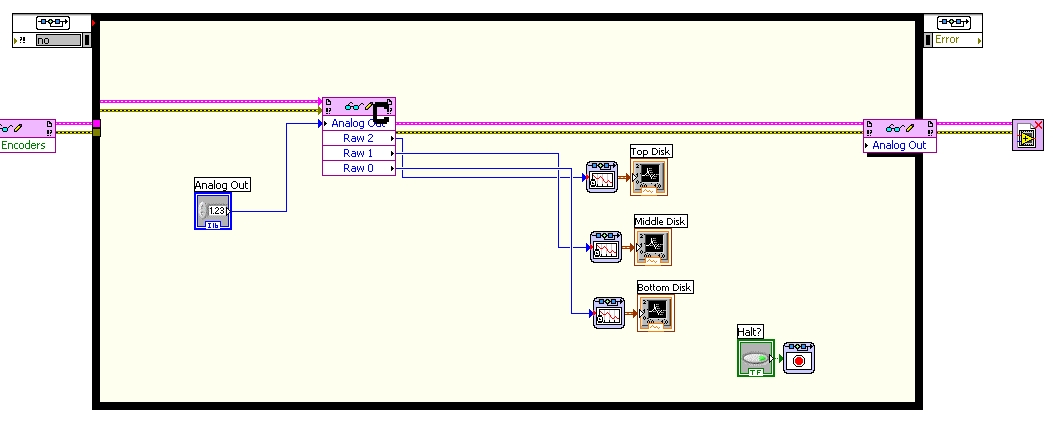
\includegraphics[width=6in]{Lab3/fpgatemplate}
\caption{The template you will be using}
\label{fig-vitemplate}
\end{figure}


All of the FPGA code for this lab and most (possibly all) of the subsequent labs
will be written for you and loaded onto the boards in advance.  

Template vi's, in normal LabVIEW for windows, have been created for your use in
this lab.  To use them, go to {\tt Desktop--Modules--ECEN Control
  Systems--Torsional Interface} and copy the files to a directory on your
``Z''-drive.  You may rename the file ``torisonal\_plant\_template.vi'' to
whatever you wish, but do not rename the other files.

%To use them, selected {\tt VI from Template...} on the LabVIEW main window. 
%Create a VI from a {\tt VI $\to$ From Template $\to$ ECEN4638 Lab 3}.  
%You may modify this VI and save it to a new location.

%Template vi's, in normal LabVIEW for windows, have been created for your use in
%this lab.  To use them, selected {\tt VI from Template...} on the LabVIEW main window. 
%Create a VI from a {\tt VI $\to$ From Template $\to$ ECEN4638 Lab 3}.  
%You may modify this VI and save it to a new location.

When the VI is first run, LabVIEW may report a "VISA: Code Module could not be loaded."
In this case, close LabVIEW, open the "Measurement and Automation" on the desktop.  
Close the program once it is loaded and restart LabVIEW.  This should fix the error.

Since the data acquisition and analog out (which will be how you send an input
to the motor in "Hardware Gain on Torque") are within a Simulation Loop, you can
use the same vi's that you have been using to do your Simulations, i.e. step
input, simulation time graph, etc.



\vspace{0.2in}
         

\noindent Remember, if you get stuck on some part of the lab, ask your
classmates, the TA, or myself.

%\newpage


%\begin{enumerate}
%\item This damped frequency, $\omega_d$ approximates the natural frequency $\omega_n$,
%  according to:
%\begin{equation}
%\omega_{n_{d31}}=\frac{\omega_{d31}}{\sqrt{1-\zeta_{d31}^2}} \approx\omega_{d31}
%\label{eq-naturalfrequency}
%\end{equation}
%This last approximation only holds for $\zeta_{d31}$ reasonably small.  (In this
%equation the $d31$ subscript denotes disk \#3, trial \#1.) Be sure to save this
%data!
%\item Remove the four masses from the third (upper) disk and repeat steps 5
%  through 7 to obtain $d32$ for the unloaded disk. 
%\item Measure the reduction from the initial cycle amplitude $X0$ to the last
%  cycle amplitude $Xn$ for the $n$ cycles measured in Step \#8. Using relationships
%  associated with the logarithmic decrement:
%\begin{equation}
%\frac{\zeta_{d32}}{\sqrt{1-\zeta_{d31}^2}}=\frac{1}{2 \pi n} \ln
%\left(\frac{X_0}{X_n}\right) \Rightarrow \zeta_{d32}\approx\frac{1}{2 \pi n} \ln
%\left(\frac{X_0}{X_n}\right)
%\label{eq-logarithmicdecrement}
%\end{equation}
%find the damping ratio $\zeta_{d32}$ and show when this term is small the
%approximations in Eqs.~(\ref{eq-naturalfrequency}) and
%(\ref{eq-logarithmicdecrement}) hold.
%\item Repeat Step 5 through 9 for the lower disk, disk \#1. Here in Step 6 you
%  will need to remove Encoder \#3 position and add Encoder \#1 position to the
%  plot set-up. Hence obtain $\omega_{n_{d11}}$, $\omega_{n_{d12}}$, and $\zeta_{d12}$. How
%  does this damping ratio compare with that for the upper disk?
%\item Use the following information pertaining to each mass piece to calculate
%  the portion of each disk's inertia attributable to the four masses for the
%  "$d31$" and "$d11$" cases. \\
%  \begin{enumerate}
%  \item Mass (incl. bolt \& nut) = $500g$ ($\pm5g$);
%  \item  diameter = $5.00cm$  ($\pm0.02cm$);
%  \end{enumerate}


%\item Calling this inertia $J_m$. (i.e. that associated with the four masses
%  combined), use the following relationships to solve for the unloaded disk
%  inertia $J_{d3}$, and upper torsional shaft spring $k_{d3}$.
%\begin{eqnarray}
%(\omega_{n_{d31}})^2 & = & \frac{k_{d3}}{J_m+J_{d3}}\\
%(\omega_{n_{d32}})^2 & = & \frac{k_{d3}}{J_{d3}}
%\end{eqnarray}
%  Find the damping coefficient $c_{d3}$ by equating the first order terms in the
%  equation form:
%  \begin{equation}
%    \label{eq-damping}
%s^2+2\zeta\omega_ns+\omega_n^2=s^2+\frac{c}{J}s+\frac{k}{J}    
%  \end{equation}
%  Repeat this for the lower unloaded disk inertia (this includes the reflected
%  inertias of the motor, belt, and pulleys), spring and damping $J_{d1}$ ,$c_{d1}$,
%  and $k_{d1}$ respectively.
%\end{enumerate}

%Now all dynamic parameters have been identified! Values for $J_1$ and $J_2$ for any
%configuration of masses may be found by adding the calculated inertia
%contribution of the masses to that of the unloaded disk.

%\subsection{Task \#4--System Identification Results}
%Write down the values of the parameters you computed here.  

%\begin{center}
%\vspace{.2in}
%\begin{tabular}{||l|l||}
%\hline
%Variable & \hspace{2in}Value \\
%\hline
%$J_1$ & \\
%\hline
%$J_2$ & \\
%\hline
%$J_3$ & \\
%\hline
%$c_1$ & \\
%\hline
%$c_2$ & \\
%\hline
%$c_3$ & \\
%\hline
%$k_1$ & \\
%\hline
%$k_2$ & \\
%\hline
%\end{tabular}
%\vspace{.2in}
%\end{center}

%This is probably a good potential stopping point for day one.

%\subsection{Task \#3--Hardware Gain on Torque}
%The following is necessary to establish the hardware gain for control modeling
%purposes.
%\begin{enumerate}
%\item Remove the entire upper disk, unfasten the mid-shaft disk and clamp and
%  replace the four masses on the lower disk (only) at the 9.0 cm center distance
%  following the guidelines of Step 2. Verify that the masses are secure and that
%  the disk rotates freely. Hook up the drive power to the mechanism.
%\item \textbf{What voltages should we use here?}  Create an open-loop pulse that
%  is 1.00 Volts for 500 ms. To do this, you need to know that the FPGA's we are
%  using scale by a factor of 3270, so you will need to scale your input by this
%  much using a gain block.  Plot Encoder \#1.
%\item Plot this data and observe four velocity profile segments with nominal
%  shapes of: linear increase (constant acceleration), constant (zero
%  acceleration), linear decrease (deceleration), and constant. Obtain the
%  acceleration, $\ddot{\theta}_{1e}$, (counts/$s^2$) by carefully measuring the velocity difference
%  and dividing by the time difference (500 ms) through the positive-sloped
%  linear segment.  Repeat this for the negative-sloped segment. 
%\end{enumerate}

%You now have enough information to  determine the hardware gain $k_{hw}$.
%Decide on a method of using this data to determine $k_{hw}$ and compute accordingly.



%\subsection{Task \#5--System Identification Analysis}

%You now have a nominally identified system!  The question is whether these
%parameters are enough to give you a good model of what the system
%\emph{actually} does.  

%\noindent \textbf{Task:}  Use your state-space implementation
%of the system to simulate the system with the correct parameters you have just
%computed.

%\noindent \textbf{Task:}  Design two experiments that you can use to verify your
%model against the experiment.  One should involve no applied torque (just
%setting the intial conditions) and the other should involve an applied torque.  

%\noindent \textbf{Task:}  How close is your model to the real system?  Describe
%what differences there are. Can they be fixed?  If not, how will they affect the
%controller design?

%\begin{center}
%\framebox{\parbox{4in}{
%This problem is open-ended.  You need to justify to the best of your ability the
%fact that your model adequately represents the real system.  }}
%\end{center}









%% Local Variables:
%% TeX-master: "../LVmanual.tex"
%% End:
